\documentclass{article}

\usepackage[preprint]{neurips_2026}
\makeatletter
\renewcommand{\@noticestring}{MAS.S62 Self-Evolving AI, Fall 2026: project proposal}
\makeatother

\usepackage[utf8]{inputenc}
\usepackage[T1]{fontenc}
\usepackage{hyperref}
\usepackage{url}
\usepackage{booktabs}
\usepackage{amsfonts}
\usepackage{nicefrac}
\usepackage{microtype}
\usepackage{xcolor}
\usepackage{tikz}
\usetikzlibrary{positioning,fit,arrows.meta,backgrounds,calc}
\usepackage{enumitem}
\usepackage{tabularx}
\setlist{nosep, leftmargin=*}

\definecolor{ink}{HTML}{1F2933}
\definecolor{rule}{HTML}{2F6F4E}
\definecolor{opt}{HTML}{3B5B92}
\definecolor{bad}{HTML}{B4442E}
\definecolor{soft}{HTML}{F3F5F4}
\hypersetup{colorlinks=true, linkcolor=opt, citecolor=opt, urlcolor=opt}

\newcommand{\dec}{\textsc{Decorum}}
\newcommand{\RQ}[1]{\textbf{RQ#1}}

\title{\dec: Evolving the Rules, Not the Graph,\\of Multi-Agent Collaboration}

\author{%
  Anthony Baez \qquad Max Holschneider \qquad Tawab Safi\\
  MAS.S62 Self-Evolving AI\\
  \texttt{\href{https://github.com/asaficontact/decorum}{github.com/asaficontact/decorum}}
}

\begin{document}

\maketitle

\begin{abstract}
Coding agents now work as teams in which a main agent spawns and delegates to subagents, yet automated team design searches over \emph{who talks to whom}: graphs, workflows, rosters.
We propose \dec, which evolves \emph{how agents talk}: a typed, domain-agnostic \emph{rulebook} (visibility, handoff, closing with evidence, review, dissent, escalation, budget) for a forum of threads and tasks managed by the main agent.
The harness enforces the rules through tools and hooks; the topology emerges at run time; a reflective optimizer edits the rulebook from scores, threads and traces.
We test whether an evolved rulebook (i)~solves more held-out coding tasks than hand-designed topologies at equal budget, (ii)~degrades less with a saboteur or prompt-injected subagent, and whether enforcement is what protects it, and (iii)~transfers zero-shot to multi-hop research; and (iv)~which evidence the optimizer needs.
\end{abstract}

\section{Introduction}

Multi-agent harnesses are now a common way to run long agentic tasks, but their agents do not yet know how to collaborate.
Anthropic's swarm experiments surface three failures: conformity, a lack of epistemic rigor, and incompatible goals.
They also find that prescribing roles or a ``CEO'' hierarchy in the prompt made little difference, and call for norms built for agents~\citep{anthropic2026patterns}.
Across 1{,}600+ traces from seven frameworks, failures split into system design (41.8\%), inter-agent misalignment (36.9\%) and task verification (21.3\%), and changing the system design alone moved success~\citep{cemri2025why}.
Structure decides outcomes: across 260 controlled configurations, architecture changes performance relative to a single agent by anywhere from $+80.8\%$ to $-70.0\%$~\citep{kim2025towards}. Even hand-designed governance matters: run as agent architectures, the best of seven historical institutions beats a single agent by 8--57 points across two benchmarks~\citep{fei2026when}.

Automated multi-agent design has mostly searched over \emph{structure}: graphs, workflow code, architectures and prompts (\S2).
Two things are missing.
First, the failures above concern \emph{conduct}, not wiring: who may read what and when, what counts as done, who must review, and how dissent is surfaced.
Second, in real coding harnesses the main agent decides at run time whom to spawn and what to hand over; run-time methods optimize that orchestrator~\citep{dang2025multi,ruan2026aorchestra}, not the rules its subagents follow.

\dec{} treats the \emph{rules of interaction} as the object of evolution (Fig.~\ref{fig:decorum}).
The main agent manages a forum: each task has a thread holding its full discussion, which several subagents may share and a successor inherits. A YAML rulebook of typed primitives, compiled into tool gates and hooks, governs the forum; the main agent stays free to choose the topology.
Rules stated only in prompts decay over long contexts~\citep{gamage2026omission} and get lost in delegation: with a 32B model, 85\% of policy-relevant facts are dropped at orchestrator--subagent handoff vs.\ 0\% in a single loop~\citep{li2026governance}.
We therefore separate enforced rules from a prompt-only \texttt{norms:} field.

\textbf{Broad impact.} Agent teams already edit code and act on the web; enforced rules make them auditable, and threads give humans one readable record per task instead of thousands of traces.
\textbf{Intellectual merit.} It is open whether the \emph{rules} of a collaboration are a better search space than hand-designed (and, ultimately, evolved) \emph{graphs}, whether rules found for performance are robust to bad actors (optimizing for capability alone erodes safety~\citep{shao2026your,rosser2025agentbreeder}), and whether conduct transfers across domains when structure does not.
\textbf{Technical challenges.} Compiling rules into hooks without blocking valid work; blaming one rule for a failure in a long thread; evaluating edits on noisy, costly runs; and keeping enforced and prompted arms information-matched.

\begin{figure}[t]
\centering
\resizebox{0.8\linewidth}{!}{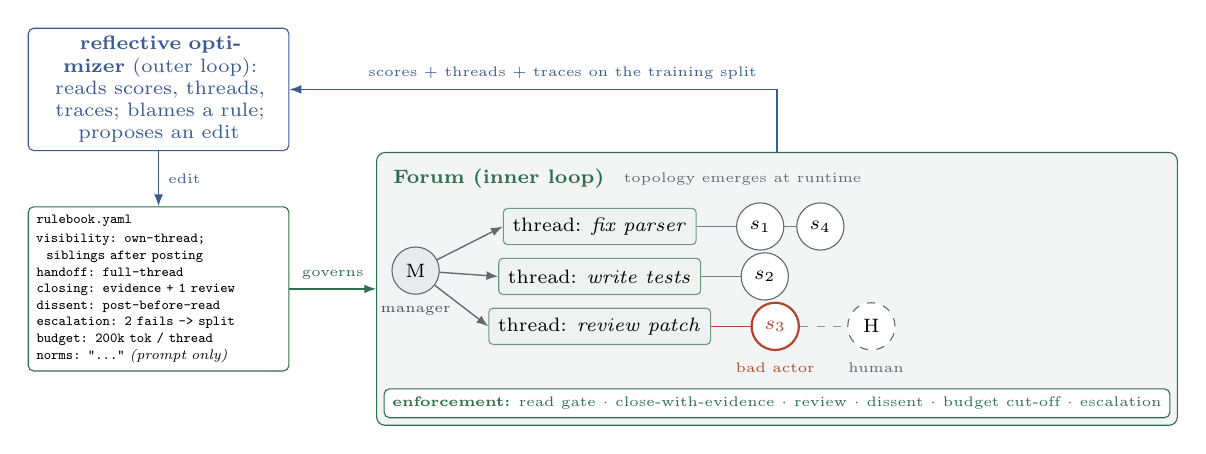
\begin{tikzpicture}[font=\scriptsize, node distance=3mm,
  box/.style={draw=ink!60, rounded corners=2pt, fill=white, inner sep=3pt, align=center},
  agent/.style={draw=ink!70, circle, minimum size=6mm, inner sep=0pt, fill=white},
  thr/.style={draw=rule!70, rounded corners=1.5pt, fill=rule!8, minimum width=21mm, minimum height=4.6mm, align=center},
  arr/.style={-{Latex[length=1.5mm]}, draw=ink!70, line width=0.5pt}]
% ---- forum ----
\node[agent, fill=ink!10] (M) {M};
\node[below=0.3mm of M, font=\tiny, text=ink!80] {manager};
\node[thr, right=8mm of M, yshift=5.6mm] (T1) {thread: \emph{fix parser}};
\node[thr, below=1.6mm of T1] (T2) {thread: \emph{write tests}};
\node[thr, below=1.6mm of T2] (T3) {thread: \emph{review patch}};
\node[agent, right=5mm of T1] (S1) {$s_1$};
\node[agent, right=1.5mm of S1] (S4) {$s_4$};
\node[agent, right=5mm of T2] (S2) {$s_2$};
\node[agent, right=5mm of T3, draw=bad, text=bad, thick] (S3) {$s_3$};
\node[agent, right=6mm of S3, dashed] (H) {H};
\draw[arr] (M) -- (T1.west); \draw[arr] (M) -- (T2.west); \draw[arr] (M) -- (T3.west);
\draw[ink!60] (T1) -- (S1); \draw[ink!60] (S1) -- (S4); \draw[ink!60] (T2) -- (S2);
\draw[bad] (T3) -- (S3); \draw[ink!50, dashed] (S3) -- (H);
\node[font=\tiny, text=bad, anchor=north] at ($(S3.south)+(0,-0.3mm)$) {bad actor};
\node[font=\tiny, text=ink!70, anchor=north] at ($(H.south)+(0.6mm,-0.3mm)$) {human};
\node[box, draw=rule, text=rule, fill=white, font=\tiny, anchor=north west, minimum width=0pt] (E) at ($(M.west|-T3.south)+(-1mm,-5.5mm)$)
  {\textbf{enforcement:} read gate $\cdot$ close-with-evidence $\cdot$ review $\cdot$ dissent $\cdot$ budget cut-off $\cdot$ escalation};
\node[font=\scriptsize\bfseries, text=rule, anchor=south west] (FL) at ($(M.west|-T1.north)+(-1mm,1.2mm)$) {Forum (inner loop)};
\node[font=\tiny, text=ink!70, anchor=west] at (FL.east) {topology emerges at runtime};
\begin{scope}[on background layer]
\node[draw=rule, fill=soft, rounded corners=3pt, inner sep=2.5pt, fit=(FL)(M)(T1)(T3)(S4)(H)(E)] (F) {};
\end{scope}
% ---- rulebook ----
\node[box, draw=rule, anchor=east, text width=31mm, align=left, font=\tiny\ttfamily] (R) at ($(F.west)+(-11mm,0)$) {%
\textbf{rulebook.yaml}\\[1pt]
visibility: own-thread;\\\ \ siblings after posting\\
handoff: full-thread\\
closing: evidence + 1 review\\
dissent: post-before-read\\
escalation: 2 fails -> split\\
budget: 200k tok / thread\\
norms: "..." \textrm{\textit{(prompt only)}}};
\draw[arr, draw=rule] (R.east) -- node[above, font=\tiny, text=rule]{governs} (F.west|-R.east);
% ---- optimizer ----
\node[box, draw=opt, text=opt, anchor=south, text width=31mm] (O) at ($(R.north)+(0,7mm)$) {\textbf{reflective optimizer} (outer loop): reads scores, threads, traces; blames a rule; proposes an edit};
\draw[arr, draw=opt] (O) -- node[right, font=\tiny, text=opt]{edit} (R);
\draw[arr, draw=opt] (F.north) |- node[pos=0.72, above, font=\tiny, text=opt]{scores $+$ threads $+$ traces on the training split} (O.east);
\end{tikzpicture}
}
\caption{\dec. The main agent (M) opens a thread per task and assigns subagents ($s_i$); the topology is never written down. Typed primitives compile into an enforcement layer; \texttt{norms:} is prompt-only. A reflective optimizer edits the rulebook from training runs. At test time one subagent may be a saboteur or injected (red); a human may join (stretch).}
\label{fig:decorum}
\end{figure}

\section{Related work}

\textbf{Searching over topologies and workflows.}
GPTSwarm optimizes agent graphs~\citep{zhuge2024gptswarm}, and G-Designer and MaAS generate query-conditioned topologies and architectures~\citep{zhang2025gdesigner,zhang2025multi}.
ADAS and AFlow search over agent and workflow code~\citep{hu2025automated,zhang2025aflow}, and MASS interleaves prompt and topology search~\citep{zhou2026multi}.
Puppeteer, AOrchestra and MANTA choose the topology at run time~\citep{dang2025multi,ruan2026aorchestra,huang2026manta}.
\emph{Limitation:} the optimized artifact is a structure (or, at run time, the orchestrator itself); coordination rules, when they exist, are prompt text or control flow baked into it, and found systems transfer poorly (AgentDropout: $63.5\%\rightarrow55.8\%$ out of domain~\citep{so2026superficial}).

\textbf{Coordination substrates, norms and evolved constitutions.}
Hand-designed substrates include SOPs with a shared message pool~\citep{hong2024metagpt}, ledgers~\citep{fourney2024magentic} and negotiated protocols~\citep{marro2024scalable}.
Normative multi-agent systems and electronic institutions have long enforced interaction rules through infrastructure~\citep{esteva2001formal,boella2006introduction}, and a hand-written dissent-style protocol sharply raises hidden-profile accuracy~\citep{li2026systematic}.
A 2026 cluster evolves natural-language \emph{constitutions} for agent societies~\citep{kumar2026evolving,niranjani2026internal} or teams~\citep{hao2026evolve}, and proposes portable self-evolving coordination specifications~\citep{zhang2026swarm}.
\emph{Limitation:} evolved rules are prompt-level, evaluated in toy games or within one benchmark, and never tested against an adversarial teammate or across task domains.

\textbf{Reflective optimization from traces.}
TextGrad, Trace and GEPA have an LLM read execution feedback and edit text artifacts~\citep{yuksekgonul2025optimizing,cheng2024trace,agrawal2026gepa}.
Meta-Harness extends this to harness code; in its one-domain ablation, raw traces beat scores alone (median $50.0$ vs.\ $34.6$), while LLM summaries recover none of the gap ($34.9$)~\citep{lee2026metaharness}.
\emph{Limitation:} gains often vanish against matched-compute baselines or on held-out tasks~\citep{wang2026rethinking}, design cost rarely pays off~\citep{el2025inefficiencies}, and the one trace-driven method that edits inter-agent rules (Meta-Team) edits prompt text by team self-reflection~\citep{hao2026evolve}.

\textbf{Safety under bad actors, and enforcement.}
LLM teams degrade with faulty members~\citep{huang2025resilience}, injections spread between agents~\citep{lee2024prompt}, and code injection compromises coding teams~\citep{bowers2025analyzing}.
AgentBreeder, MaMa and SHE evolve scaffolds, systems or a single agent's harness for safety~\citep{rosser2025agentbreeder,nother2026mama,qu2026she}.
On enforcement, an enforced governance manifest cut severe collusion from 50\% to 5.6\% where the same rules as a prompt did not~\citep{bracalesyrnikov2026institutional}.
On short delegation chains, however, a strong prompt ties enforcement (POLIS~\citep{x2026multi}), and runtime-enforced organizations can still lose to a single agent~\citep{hsu2026opencollab}.
\emph{Limitation:} enforced inter-agent rules are hand-written (MaMa's optional per-environment tools aside; SHE evolves enforced rules for a single agent), and enforced vs.\ prompted rules have not been compared in cooperative, long-horizon teams under attack.

\textbf{Closest work.}
\emph{Meta-Team}~\citep{hao2026evolve} evolves a team constitution, profiles and roster by self-reflection in a harness that recruits agents at run time.
On nine coding, research, GAIA and long-context columns it averages $62.7$ vs.\ $56.1$ for the unevolved team.
Its constitution is prompt text, it has no adversaries, and its out-of-distribution tests stay within one benchmark.
\emph{Constitutional Evolution}~\citep{kumar2026evolving} evolves prompt-level norms for six agents in a grid-world survival game, scoring $0.556$ vs.\ $0.249$ for human-written norms, with no task solving, topology baseline or transfer.
\emph{AgentBreeder}~\citep{rosser2025agentbreeder} evolves multi-agent Python scaffolds for capability and safety (blue mode: $+79.4\%$ safety on average), but safety means refusing harmful user prompts in single-turn QA; no agent inside the system is compromised.
\dec{} differs in the combination: a typed rulebook, enforced by the harness and domain-agnostic, evolved by an outer optimizer for task success; topology left to the main agent; robustness tested against saboteur and injected teammates; and transfer tested across task domains.

\begin{table}[b]
\centering
\footnotesize
\setlength{\tabcolsep}{4pt}
\caption{Conditions, all at the same model and per-instance token cap. E1--E4 answer RQ1--RQ4 (performance, safety, transfer, optimizer input). $\dagger$: stretch.}
\label{tab:conditions}
\begin{tabularx}{\linewidth}{@{}lXl@{}}
\toprule
Condition & What varies & Used in \\
\midrule
Single agent & one agent, same budget (the floor, and the task-selection test) & E1, E3 \\
Default harness & main agent with subagents and file/message handoff; no forum & E1 \\
Fixed topologies & star, chain, debate, review loop: fixed graphs in the same harness, forum off & E1--E3 \\
Default rulebook & our hand-written rulebook, not evolved & E1--E3 \\
Evolved \texttt{norms:} only & prompt-only rules evolved (a Meta-Team-style baseline) & E1, E2 \\
\textbf{Evolved rulebook} & \textbf{enforced primitives and norms, evolved} & E1--E4 \\
Evolved rulebook, prompted & same rule text, nothing enforced & E2 \\
Best-of-$N$ at matched compute & sampling instead of evolution~\citep{wang2026rethinking} & E1 \\
Research-evolved rulebook & evolved in-domain on research (transfer ceiling) & E3 \\
Evolved graph$^\dagger$ & same optimizer, searching over roles and edges & E1--E3 \\
\bottomrule
\end{tabularx}
\end{table}

\section{Research ideas}

The three ideas share one harness; each will be led by one team member (leads to be assigned).

\textbf{Idea 1: Evolving an enforced rulebook (\RQ{1}, \RQ{4}).}
Build the forum and a rulebook of seven typed primitives (Fig.~\ref{fig:decorum}), each compiled into enforcement code with a prompt-only twin.
A GEPA-style optimizer~\citep{agrawal2026gepa} reads failed threads, attributes failure to a rule, proposes an edit, and accepts it only if it holds up on a validation split.
\RQ{1}: does an evolved rulebook beat the default rulebook and the best hand-designed topologies at equal budget?
\RQ{4}: does the optimizer need threads and traces, or do scores suffice? \emph{Novelty:} prior evolved rules are prompt-level~\citep{hao2026evolve,kumar2026evolving}; ours are enforced and compared with topologies.

\textbf{Idea 2: Enforced rules under bad actors (\RQ{2}).}
At test time one subagent is either a \emph{saboteur} (instructed to slip in a subtle bug or a false claim with fabricated evidence) or \emph{injected} (turned by a poisoned file in the repository).
The main agent is trusted and does not know which subagent is bad.
\RQ{2}: are rules evolved only for performance more robust than topologies, and is enforcement, not rule content, what protects them?
\emph{Novelty:} AgentBreeder and MaMa evolve \emph{for} safety; we test performance-evolved rules against in-team saboteurs and injection, enforced vs.\ prompted. \emph{Stretch:} adversaries also during evolution (as in AgentBreeder's blue mode).

\textbf{Idea 3: Transfer and growth of the rulebook (\RQ{3}).}
Primitives speak of \emph{evidence}, \emph{review} and \emph{handoff}, so a coding-evolved rulebook runs unchanged on research; an adapter maps evidence to passing tests or to quoted sources.
\RQ{3}: what share of the gap from the default to a research-evolved rulebook does the transferred one close, and do rules transfer better than topologies? \emph{Novelty:} searched systems transfer poorly~\citep{huang2026manta,so2026superficial}, and evolved \emph{rules} have never been moved across domains.
\emph{Stretch:} (a)~the optimizer writes and tests \emph{new} enforcement primitives, seeded by ideas it keeps writing into \texttt{norms:}; (b)~a \emph{human joins the forum} under an evolvable, budgeted \texttt{escalation\_to\_human} rule, scored by recovery per intervention with a simulated oracle, then a small real-human pilot (simulators overstate success: 63.6\% real vs.\ up to 77.8\%~\citep{zhou2026mind}). Prior escalation policies are hand-written or learned in weights~\citep{mozannar2025magentic,yang2026adaptive,feng2024large}.

\section{Planned execution}

\textbf{Datasets.}
\emph{Coding} (evolve and test): candidates must be hard for one agent at equal budget, decomposable, scored by executed tests, and splittable by repository. The current lead is SWE-rebench~\citep{badertdinov2025swerebench} (21{,}336 tasks from 3{,}468 repositories, with monthly fresh splits): evolve on 60--100 tasks, test on 100--150 from unseen repositories.
Alternatives: SWE-bench Pro~\citep{deng2025swebench}, DeepSWE~\citep{huang2026deepswe}; not SWE-bench Verified (59.4\% of 138 audited hard tasks had flawed tests~\citep{openai2026noverified}).
\emph{Research} (transfer; one in-domain run as RQ3 ceiling): BrowseComp-Plus~\citep{chen2025browsecompplus}, 830 questions over a fixed 100{,}195-document corpus; we validate its judge on 100 hand-labelled answers. We avoid closed-book multi-hop sets, where one agent matches multi-agent systems at equal budget~\citep{tran2026single}.
\emph{Threats:} saboteur and injection suites adapted from ORBIT, SHADE-Arena and code-injection attacks~\citep{hagag2026orbit,kutasov2025shade,bowers2025analyzing}.

\textbf{Metrics.}
\emph{Task:} resolve rate (hidden tests pass) and answer accuracy at a harness-enforced per-instance token cap.
\emph{Cost:} tokens, time, and the optimizer's own spend.
\emph{Safety:} clean success, success under attack, attack success (the bug or false claim is merged), detection (the bad actor is flagged).
\emph{Mechanism:} adherence (the run did what the rulebook said~\citep{hsu2026opencollab}); attempted vs.\ realized violations.
\emph{Transfer:} share of the default-to-ceiling gap closed. \emph{Qualitative:} which primitives evolution keeps; threads read by hand per failure class.


\textbf{Experimental setup.}
Agents run on Pi (Claude Agent SDK as fallback), whose tool-call hooks can block or rewrite actions.
\emph{E1} compares Table~\ref{tab:conditions}'s conditions on held-out coding; \emph{E2} replays them with a saboteur or injected subagent; \emph{E3} runs the coding-evolved rulebook zero-shot on research; \emph{E4} feeds the optimizer scores, $+$threads, or $+$threads$+$traces.
Controls: shuffled \texttt{norms:} (content vs.\ priming); emergent topology replayed with random rules (rules vs.\ graph).
Reruns can flip 5 of 36 tasks~\citep{hsu2026opencollab}, so baselines run twice (noise floor) with paired bootstrap CIs.
\emph{Hypotheses:} the evolved rulebook beats the best fixed topology (E1), loses less under attack with enforced ahead of prompted (E2), closes most of the transfer gap unlike fixed topologies (E3), and needs threads, not just scores (E4).
\emph{Kill conditions} (fixed in advance): one agent matches the teams (change the task); evolved $\approx$ default rulebook (evolution adds nothing); no win over the best fixed topology (RQ1 fails); enforced $\approx$ prompted under attack (enforcement is not the mechanism).

\textbf{Risks and mitigations.}
\emph{Cost:} small subsets, a cheaper model for evolution, per-thread caps, optimizer spend reported.
\emph{Overfitting:} repository-disjoint splits, matched-compute baseline. \emph{Reward hacking} (winning by refusing or closing early): clean success and adherence reported for every rulebook~\citep{rosser2025agentbreeder}.
\emph{Over-blocking:} refusals say what is missing. \emph{Build risk:} Pi lacks built-in subagents; we add them as an extension (fallback: Claude Agent SDK).
\emph{Unsafe drift:} attack success reported for every accepted rulebook.

\textbf{Stretch goals} (priority order): evolved graph; adversaries in evolution; new primitives; human escalation; poor collaborators.

\textbf{Team and timeline.}
In October the work splits into three packages, one owner each and reviewed by a second member: the forum and enforcement layer (threads, tasks, hooks, prompted twins); the evaluation harness (benchmarks, repository splits, cost caps, attack suites, logging); and the optimizer (failure attribution, edits, validation gate). From November each member leads one idea (Idea~1: [lead TBD]; Idea~2: [lead TBD]; Idea~3: [lead TBD]) and reviews another's runs.
\emph{Oct 5--18:} harness, primitives v0, benchmarks, 20 tasks read, single-agent baseline twice.
\emph{Oct 19--Nov 1:} default rulebook, prompted twins, fixed topologies, E1 baselines, optimizer v0.
\emph{Nov 2--15:} evolution (E1), optimizer-input ablation (E4), attack suites.
\emph{Nov 16--29:} safety (E2) and transfer (E3).
\emph{Nov 30--Dec 13:} stretch goals; final report and presentation.

\bibliographystyle{plainnat}
\bibliography{references}

\end{document}
